% \begin{frame}
%     \frametitle{Table of Contents}
%     \tableofcontents[currentsection]
% \end{frame}


% \AtBeginSection[]
% % \AtBeginSection[]{intro}
% {

% }


    %in comparison with other methods which offered improvements by \SI{56.4}{\percent} and \SI{21.2}{\percent} for the max number of \glspl{gb} reported and relative to their own constant, average models. %Additionally, octonions are symmetrized $\sim$5 orders of magnitude faster than the traditional octonion approach.
    %A \gls{gprm} model is also developed and applied for the Fe simulation dataset, yielding a simulation-based interpolation function for Fe \gls{gbe} with quantified uncertainty.
    
    
    % %%Graphical abstract
% \begin{graphicalabstract}
% 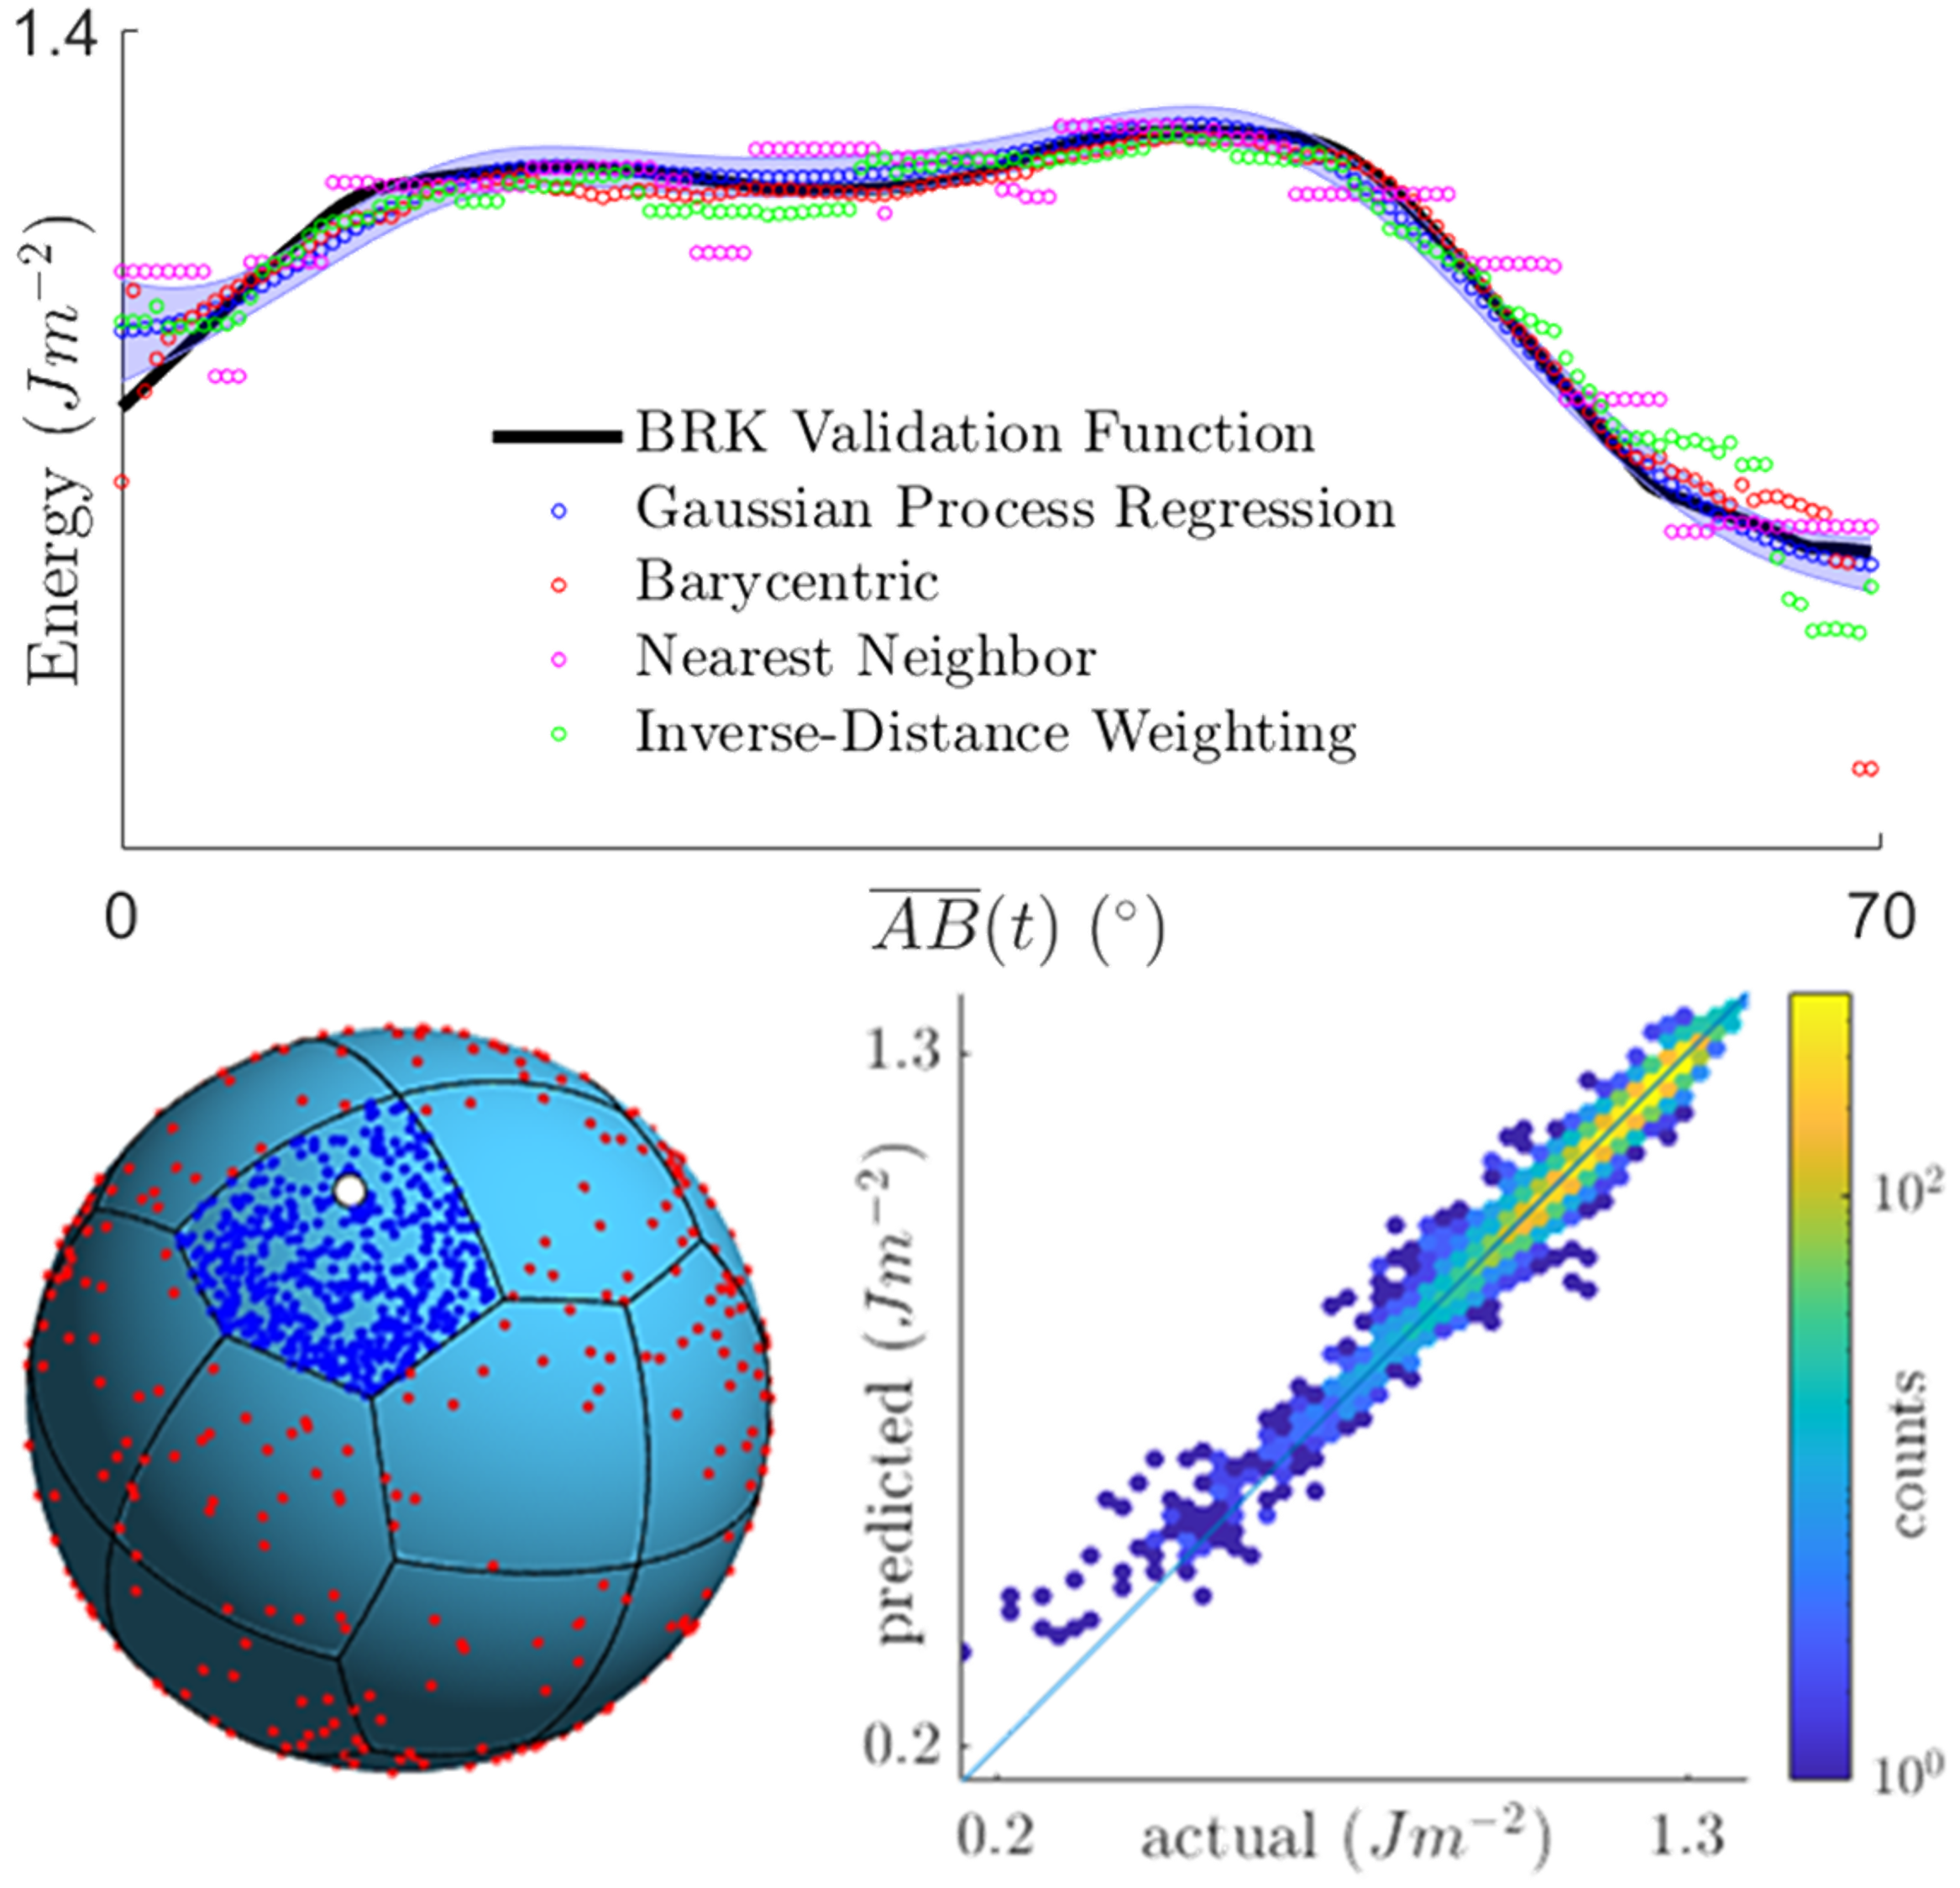
\includegraphics[width=130mm]{abstract.png}
% \end{graphicalabstract}

% \glsresetall %reset the abbreviations


 %We present the first \gls{fz} that incorporates the full \gls{5dof} \gls{gbc} in continuous coordinates which we will refer to as a \gls{vfz}. %Rather than defining a 5DOF GB \gls{fz} using linear inequalities which is the traditional approach that has been applied to other crystallographic spaces (e.g. the orientation \cite{heinzRepresentationOrientationDisorientation1991} and misorientation \cite{grimmerUniqueDescriptionRelative1980,heinzRepresentationOrientationDisorientation1991} \glspl{fz}), we employ a numerical strategy to define what we will refer to as a \gls{vfz}.

%(\citet{bulatovGrainBoundaryEnergy2014}) %(\citet{kimPhasefieldModeling3D2014}) %(\citet{olmstedSurveyComputedGrain2009})
    
 %Using the traditional octonion approach, we estimate the computation of a symmetrized $\num{50000}\times\num{50000}$ pairwise distance matrix to take \num{300} CPU days. By contrast, we compute a symmetrized pairwise distance matrix of the same size in approximately one minute. %and compare these against a constant, average model % (\gls{rmse} $\simeq$ \SI{\avgrmse{}}{\J\per\square\meter}). This gives \gls{rmse} values of \baryrmse{}, \gprrmse{}, \idwrmse{}, and \SI{\nnrmse{}}{\J\per\square\meter},
    %, 0.063, 0.056, 0.068, and \SI{0.082}{\J\per\square\meter}, respectively,

% Explain the "voronoi" type definition of the vfz by choosing a reference GB and then taking the symmetric image of each GB that is closest to that reference GB. You will need to convince the reader (probably by reason, or proof, or numerical tests) that the resulting vfz does in fact contain one and ONLY one SEO for every GB (i.e. that it does satisfy the definition of a FZ). This is probably where you note that for it to work, the reference GB needs to be something that isn't a high-symmetry GB, and why. This discussion will probably benefit from a figure illustrating the procedure in 2D.
%, as described in \cref{sec:results:accuracy}, and that overall errors will remain low as shown in \cref{fig:brkerror}, and \cref{tab:rmse-error-comparison,tab:mae-error-comparison}.


%matrix multiplication
% \begin{equation}
%     \label{eq:bary-interp_multi}
%     \mathbf{v}_q = \Lambda \mathbf{v}_m
% \end{equation}
% where $\mathbf{v}_m$ is the vector of GB properties at the mesh vertices, $\Lambda$ is the sparse matrix whose rows contain the barycentric weights for each query point, and $\mathbf{v}_q$ is the vector containing the interpolated properties at the query points.

% Give brief explanation of standard barycentric interpolation: you find which simplex the point is in, then you calculate the weights. The advantage of this approach is that the weight matrix only has to be computed once. If you interpolate different functions over the same query points, the weights don't change, so re-evaluation with a new function is rapid via a simple matrix multiplication.

% Explain how to adapt barycentric interpolation to the vfz: how to identify which simplex the query point falls in, and then how to compute the weights. Also explain and justify why you can use euclidean distances (i.e. because the vfz occupies a small portion of the 7-sphere it is nearly planar so euclidean distances and octonion distances are approximately equal and you can show tha figure here), and how that speeds things up.

% You don't need to give a detailed explanation of GPR, but you do need 1 sentence summarizing the idea and then point to REF for a general treatment. Explain any assumptions or adaptations that need to be done to use it with the vfz (e.g. presumably GPR is not actually operating on the surface of the 7-sphere, rather it is actually operating on all of $\mathbb{R}^8$, but because the vfz occupies a small portion of the 7-sphere it is nearly planar so euclidean distances and octonion distances are approximately equal, as mentioned previously, so it works without modification). Finally just explain that we used matlab's built-in \matlab{fitrgp()} function and the options used like you already have written.

% Explain the idea behind IDW in 1 sentence, then give the details of how you implemented it and any adaptations that are necessary for the present situation.


% Again, explain the idea in 1 sentence, and then give any special adaptations necessary.

%For a given trial run, an \inpt{} \gls{vfzo} set, \matlab{o}, and a \outpt{} \gls{vfzo} set, \matlab{o2}, are randomly generated according to \cref{sec:methods:rand}. The \gls{brk} validation function is evaluated at each of these points and the values are stored in the vectors \matlab{y} and \matlab{ytrue}, respectively. \matlab{o} and \matlab{o2} are \gls{svd} transformed together into a 7D Cartesian representation, which is an optional step for \gls{gpr}, \gls{nn}, and \gls{idw}, but is required for barycentric interpolation. Finally, we use \matlab{interp5DOF.m} \cite{bairdFiveDegreeofFreedom5DOF2020} to predict the function value at the \outpt{} points, which are stored in the vector \matlab{ypred}. We repeat this process for each of the interpolation methods approximately 10 times per set size, and compare the predictions, \matlab{ypred}, to the true values, \matlab{ytrue}.

%Thinking about where Dr. Fullwood's comment was coming from, we could either:
%1. include GPR results for 17176 and 388 GBs in the tables (straightforward)
%2. rerun the ANN and LKR methods for 50000 (significant effort)
%3. implement ANN and LKR as two of the methods we explore (moderate effort)
%4. leave as-is
% Personally, I lean towards 1. or 4. And I'm of the opinion that ANN might perform about on par with GPR and LKR would probably perform somewhere in-between GPR and IDW if all else is held constant. Just train of thought here, we don't really know if GPR would perform better than ANN or LKR (all things held constant), but rather the use of different methods provides evidence that we're doing things right (i.e. we're less likely to have fundamental errors in our computational approach).

%, except in the case of \gls{lobpcg} which used the mean of the true \gls{gbe} values instead. Additionally, \gls{lobpcg}$^*$ is not interpolation, but rather a complementary technique of reconstruction of specific \glspl{gbe} using polycrystalline data. 

%, except in the case of \gls{lobpcg}$^*$ which used the mean of the true \gls{gbe} values instead. Additionally, \gls{lobpcg} is not interpolation, but rather a complementary technique of reconstruction of specific \glspl{gbe} using polycrystalline data.

% \begin{table}
% \caption{Comparison of average runtime for each interpolation method in the present work, using \num{50000} points in the definition of the \gls{vfz}. Comparison to the work of other authors is also included. A constant model, whose value was chosen to be the mean of \matlab{f\_v}, was used as a control.}
% \centering
% \begin{tabular}{lccc}
% \toprule
% Method & \# \glspl{gb} & Runtime (\SI{}{seconds}) \\
% \midrule
% \Gls{gpr} & x & x \\
% Barycentric & x & x \\
% \gls{idw} & x & x \\
% \gls{nn} & x & x \\
% Constant & 0.13 & 0.097 \\
% LOBPCG \cite{shenDeterminingGrainBoundary2019} & 0.01--0.03 & --- \\
% ANN \cite{restrepoUsingArtificialNeural2014} & --- & 0.05--0.09 \\
% LKR \cite{chesserLearningGrainBoundary2020} & 0.0977 & --- \\
% \bottomrule
% \end{tabular}
% \label{tab:runtime-comparison}
% \end{table}

%( However, this may be computationally infeasible for large mesh sizes.

% While not implemented in this work, it is expected that an \gls{ann} such as in \cite{restrepoUsingArtificialNeural2014} could lead to even lower interpolation error than \gls{gpr} for large mesh sizes. % (e.g. https://www.mathworks.com/help/deeplearning/ref/narxnet.html, https://www.mathworks.com/help/deeplearning/function-approximation-and-nonlinear-regression.html)

%For the Fe simulation dataset, we obtain a \gls{rmse} and \gls{mae} of \SIlist{0.0405;}, respectively. For the Ni simulation dataset, we obtain a \gls{rmse} and \gls{mae} of \SIlist{0.0951;0.0622}{\J\per\square\m}, respectively.

%If multiple metastable \glspl{gbe} (e.g. 3-10 metastable states per distinct \gls{gb} rather than a single metastable \gls{gbe}) were available and/or the \glspl{gb} were sampled more uniformly in \gls{5dof} space, the \gls{gpr} mixing scheme may not have been needed to improve predictive performance of low \glspl{gbe}. For example, \gls{gpr} in \cref{fig:brkparity50000}a shows reasonable predictive performance of low \glspl{gbe}, but the \glspl{gb} are more uniformly sampled and the \inpt{} and \outpt{} data are noise-free (compare with the poor predictions for low \gls{gbe} for this data set shown in \cref{fig:kim-interp-teach}d).

% In numerical tests and consistent with our expectation, we determine that \gls{gpr} approximates the \gls{brk} validation function better than other methods when Gaussian noise is added to the training data and that parity plots have similar features to \cref{fig:kim-interp} when noise is also present in the true values. 

% where $q$ and $p$ are represented in:
% \begin{equation}q=\left(\cos \frac{\omega}{2},-P \hat{\mathbf{n}} \sin \frac{\omega}{2}\right)\end{equation}
% and
% \begin{equation}p=\left(\cos \frac{\omega}{2},-P \hat{\mathbf{n}} \sin \frac{\omega}{2}\right)\end{equation}

% In order to reduce the computationally complexity of computing barycentric coordinates in a high-dimensional space \cite{barberQuickhullAlgorithmConvex1996}, a single degenerate dimension (originally introduced by analytically minimizing $U(1)$ symmetry) is removed to enable use of MATLAB's quickhull \cite{barberQuickhullAlgorithmConvex1996} implementations such as \matlab{delaunayn} and \matlab{convhulln}. Removal of the degenerate dimension is done via a rigid \gls{svd} transformation, analogous to a Cartesian rotation and translation. Thus, a set of octonions originally represented by 8D Cartesian coordinates are collapsed to a 7D Cartesian representation while preserving both distances and angles among the points (see 3D to 2D analogue in \cref{fig:bary-remove-deg}). To further reduce the "curse of dimensionality" in computing the triangulation, a 7D Cartesian representation of the octonions constrained to lie on the surface of the 6-sphere are first projected onto a hyperplane tangent to the mean of the \inpt{} points and then rotated/translated again via \gls{svd} to produce a 6D Cartesian representation (see 3D to 2D analogue in Figure \cref{fig:bary-delaunay}). This 6D representation is used to compute a triangulation via the built-in MATLAB routine \matlab{delaunayn} based on the quickhull algorithm \cite{barberQuickhullAlgorithmConvex1996}, giving facet vertices for the 7D Cartesian hypersphere.

% To find the barycentric coordinates or weights of a \outpt{} \gls{vfzo} relative to a \gls{vfz} simplicial mesh it is necessary to first identify which simplicial facet the point is contained in and then to compute the barycentric coordinates of the point relative to the vertices of that facet. These steps are accomplished by the following approach.